Esta seção descreve mais um dos diagramas do SysML que também existem no UML. Os diagramas de caso de uso são centrais no processo de desenvolvimento de sistemas, e normalmente são desenvolvidos no início desse processo.

\subsubsection{O que são casos de uso}

Casos de uso descrevem a funcionalidade de um sistema em termos de como ele é utilizado para atingir os objetivos de seus usuários. Os usuários de um sistema são descritos como atores, que podem representar sistemas externos ou humanos que interagem com o sistema cujo caso de uso está sendo descrito.

As relações entre o sistema, seus atores e os casos de uso é, então, descrita no diagrama de casos de uso.
Casos de uso podem também ser elaborados com descrições detalhadas de seu comportamento, fazendo uso de diagramas de Atividade, de Sequência, de Contexto ou de máquinas de estado.

Um caso de uso tipicamente cobre vários cenários, que são representados como caminhos através do caso de uso, que acontecem cada um numa circunstância diferente.

\subsubsection{Estrutura dos diagramas de casos de uso}
Os diagramas de caso de uso descrevem um conjunto de atores e de casos de uso e o relacionamento entre eles.

A figura ao fim da seção mostra um exemplo de diagrama com seus principais elementos: um sistema (Surveillance System), atores, e casos de uso, além das multiplicidades dos atores e do caso de uso. 

O pacote completo do diagrama de caso de uso pode conter diagramas que descrevem mais detalhadamente cada um dos atores envolvidos no caso de uso.

A relação entre atores e casos de uso tem características como multiplicidade. A multiplicidade do caso de uso representa com quantas instâncias do caso de uso cada ator interage por vez. A multiplicidade do lado do ator representa quantos atores podem interagir com aquele caso de uso por vez.

O exemplo abaixo mostra como os casos de uso interagem entre si utilizando as palavras-chave \textit{extend} e \textit{include}.

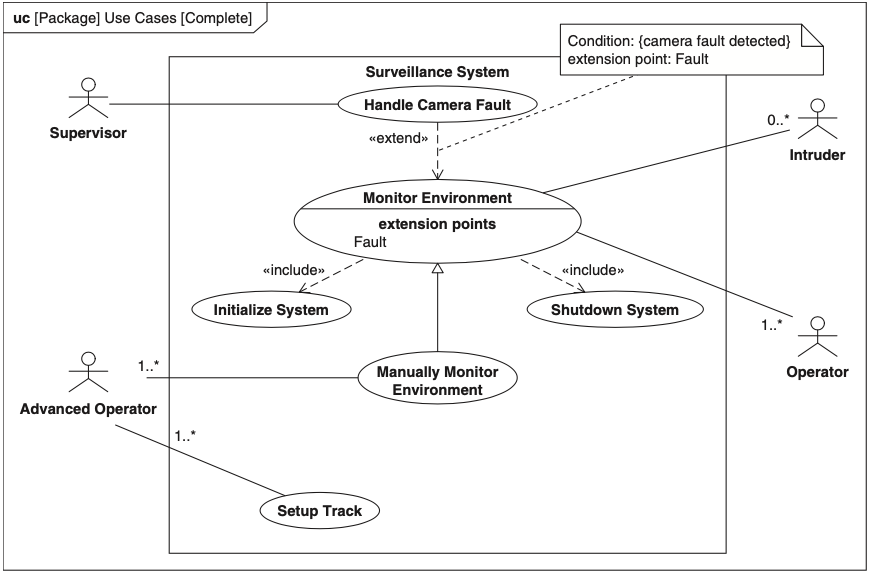
\includegraphics[width=\textwidth,height=\textheight,keepaspectratio]{figures/diagrama-caso-de-uso-3.png}

\begin{itemize}
\item \textit{include}: indica que um caso de uso utiliza a funcionalidade do caso de uso ao final da seta em algum momento do seu fluxo de trabalho. 
\item \textit{extend}: indica casos de uso que realizam alguma extensão do fluxo de trabalho do caso de uso na base da seta. 
\end{itemize}

Casos de uso também podem ser descritos de maneira textual, utilizando as palavras-chave a seguir:
\begin{itemize}
\item \textbf{Pré-Condições}: Condções necessárias para o caso de uso iniciar.
\item \textbf{Pós-Condições}: Condições necessárias após o fim da execução do caso de uso.
\item \textbf{Fluxo Primário}: Fluxo de trabalho mais frequente do caso de uso
\item \textbf{Fluxos alternativos ou de exceção}: podem existir vários, e mostram o que acontece em situações menos frequentes ou em que o sistema apresenta algum erro.
\end{itemize}

\subsubsection{Onde são utilizados com frequência}

Casos de uso são a forma principal de se descrever os requisitos para um novo software sob desenvolvimento. Eles especificam o comportamento esperado do sistema.

Assim, diagramas de caso de uso são normalmente desenvolvidos nos estágios iniciais do desenvolvimento de um sistema, e, comumente, tem o propósito de especificar o contexto do sistema, capturar os requisitos do sistema, validar a arquitetura do sistema e gerar casos de teste.

Os diagramas normalmente são desenvolvidos conjuntamente por desenvolvedores de sistemas e por \textit{experts} de domínio, nas fases iniciais de levantamento de requisitos de um sistema. 